\documentclass{article}

\usepackage{graphicx}
\usepackage{subcaption}

\graphicspath{ {phase1-files/} {phase2-files/} }

\title{CS583: Project Phase 1 and 2}
\date{\today}
\author{Serapheim Dimitropoulos}

\begin{document}

\maketitle

\section{Motivation}

Wireless sensor networks are increasingly being deployed
to measure temperature, humidity, and light and to detect
motion, fires, and landslides,among many other events of
interest. Sensors are often operated on a battery and hence
we often face a trade-off between acquiring frequent sensor
readings versus maximizing their battery life. The biggest
drainer of the battery is "communication". That is, sensors
consume the most battery power not when they sense the
environment but when they communicate their readings to a
central server.

\section{Goal}

In this project, I devised some models that try to predict
future sensor readings, given a history of past sensor
readings. The idea is that these models could potentially
be used in a central server that tries to contact
wireless sensors infrequently in order to save their
battery life. Therefore the main goal of this project
is to evaluate the devised models for use at a central
server that uses the actual readings of the sensors when
it can, and makes its own predictions when it can't
obtain the readings.

\section{General Methodology}

My data set consists of temperature and humidity readings
of 50 sensors from the Intel Berkeley Research Lab1. Since
my goal is to focus on the efficiency of my models, I make
the bold assumption that the sensor readings are not noisy
and therefore the data set that I use has been cleaned from
noisy readings. The data is divided furthermore, to train
data (used for training the models) and test data (used for
testing the models). More specifically, there are 3 days
of training data and 2 days of testing. Each day contains
48 readings per sensor (one reading taken every half hour).

For the predictions, I assumed a budget and I used two active
inference approaches: Window and Variance. By budget, I imply
that the central server can choose only a limited number
of sensor to communicate with at a time. I use this variable
in my attempt to simulate the level of frugality that the
server takes into account so as to reserve the battery of
its sensor.

The Window inference approach has the server sort the
sensor by their ID numbers and starts scanning/cycling them
for readings in that order. The amount of sensors that
the central server communicates at a time (each time stamp)
is limited by the budget mentioned earlier. The idea
behind this approach is that all sensors are guaranteed
to be read exactly once in each cycle and therefore
all of them should have about the same battery life.

The Variance inference approach is similar but with the
only difference that instead of ordering the sensors by
their ID numbers, it sorts them by their prediction variance
and choses the highest ones. Again the number of sensors
chosen is limited by the specific budget. The idea this
time is that, if a sensor's readings are known to not
vary a lot, then then probability of guessing right for
it is higher. Therefore, I want to know the exact readings
of the sensors whose readings tend to vary a lot.

Intuitively, the difference between the two approaches
seems more like a tradeoff between fairness in battery
life and accuracy as the Variance approach sounds more
accurate in terms of precision but not as fair in
preserving the battery between sensors. The reason is
that if a sensor is known to have a very high variance
in its readings then its battery will drain quicker as
the central server contacts it more often.

\section{Phase 1 Model}

In this phase I use a very simple model: each time
stamp in the day for each sensor is an independent
random variable represented as a Gaussian model with
its own mean and variance. There for the model
constructs 48 random variables for each sensor.
The mean is used as the prediction when the central
server attempts to make a guess in both approaches.
The variance of each random variable is used
to order the preference of sensor to be contacted
by the server on the Variance active inference
approach.

\section{Phase 1 Evaluation}

Assuming a variety of budgets (0, 5, 10, 20 and 25
sensors that the central server can communicate at
each time stamp), I evaluate my models by comparing
their predictions to the actual test results and
calculating the mean absolute error of my
predictions. The results are displayed in figure (a)
and (b).

\begin{figure}[h!]
	\begin{subfigure}{\linewidth}
	\includegraphics[scale=0.5]{temperature_mae.png}
	\caption{Temperature Results}
	\end{subfigure}
	\begin{subfigure}{\linewidth}
	\includegraphics[scale=0.5]{humidity_mae.png}
	\caption{Humidity Results}
	\end{subfigure}
\end{figure}

\newpage

To do some verification first, when the budget is 0
it is expected that both approaches will do equally
as is the case. Also, as the budget grows both
approaches return more accurate results which is
also expected.

In the humidity readings the Window approach is
doing slightly better than the Variance approach
which contradicts my earlier intuition. Then, the
opposite is true for the temperature readings.
The only difference is that in temperature readings
the Variance approach does better than the Window
by a slightly bigger amount than Window beats Variance
in the humidity readings. This fact, which may
be just coincidence, together with the bias of
my intuition makes me suspect that the humidity
readings triggered a lot of bad cases for my
model (many low variance sensors suddenly distancing
from the mean in the test data ...etc).

The model, although a naive one, gives descent
results on average. Nevertheless, that is the just
the average which still does not give us a lot of
insight in the efficiency of our model.

\section{Phase 2 Models}

In this phase I experiment with two models. Both use
each sensor's data as a linear chain and assume that
the states are first-order Markovian. They also
assume that the relationship between the consecutive
readings of th same sensor is Linear Gaussian. The
models do not take into account any correlation
across sensors. For learning the parameters of the
Linear Gaussian dependencies I use Linear Regression
(I fit the variance on the residuals) and for inference
simple Kalman Filtering.

The first model (Model 1) assumes that parameters
are stationary at the half-hour level, which is
also the instance of the data (0.5 hours),
while the second one (Model 2) assumes that
parameters are stationary at the day level.

In Model 1, for every sensor I estimate 5 parameters:
$\mu_i$, $\sigma_i$, $\beta_0$, $\beta_1$, and $\sigma^2$.
To estimate the last three parameters I use all data
from all days using regression and for the first two
I just use the mean and the variange again from all
the data from all the days. Knowing these, when I do
MAP assignements on the sensor data that I am trying
to predict.

In Model 2, I have 2 parameters for the initial
timestamps ($\mu_i$ and $\sigma_i$) and 3 parameters
for all the other timestamps ($\beta_0$, $\beta_1$,
and $\sigma^2$). Inference is the same in this model
with the only difference that betas change change at
every step in time.

As a final (but important) note, when I train both
the models I connect the first timestamp of the next
day with the last timestamp of the current day.

\section{Phase 2 Evaluation}

Like Phase 1,
assuming a variety of budgets (0, 5, 10, 20 and 25
sensors that the central server can communicate at
each time stamp), I evaluate my models by comparing
their predictions to the actual test results and
calculating the mean absolute error of my
predictions. The results are displayed in the figures
below.

\begin{figure}[h!]
	\begin{subfigure}{\linewidth}
	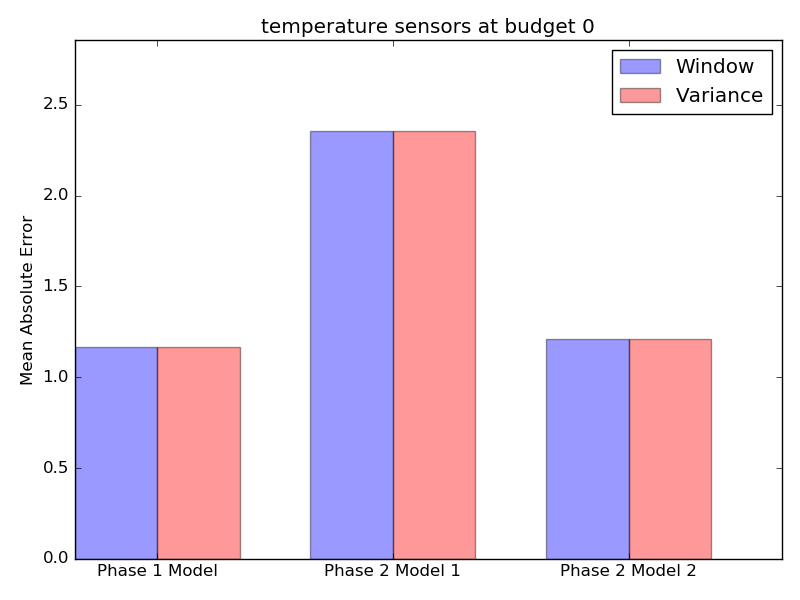
\includegraphics[scale=0.5]{temperature_0.png}
	\end{subfigure}
	\begin{subfigure}{\linewidth}
	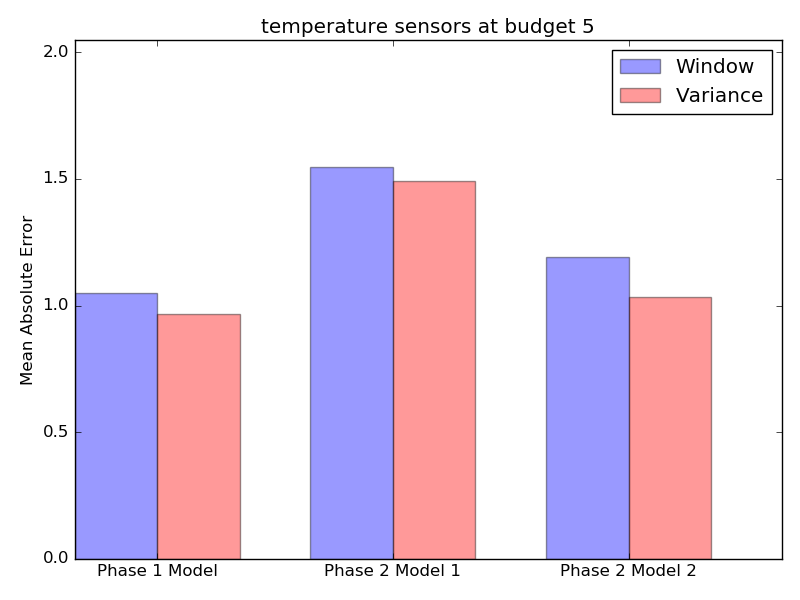
\includegraphics[scale=0.5]{temperature_5.png}
	\end{subfigure}
\end{figure}

\newpage

\begin{figure}[h!]
	\begin{subfigure}{\linewidth}
	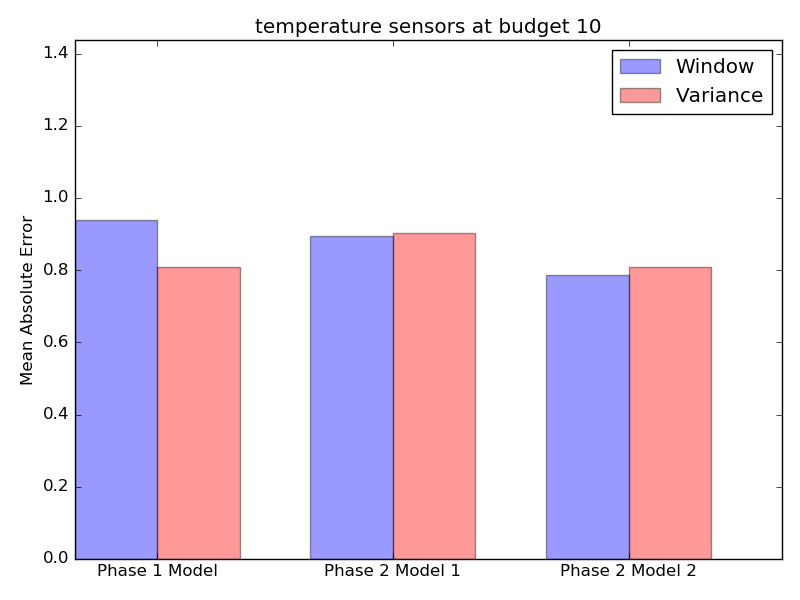
\includegraphics[scale=0.5]{temperature_10.png}
	\end{subfigure}
	\begin{subfigure}{\linewidth}
	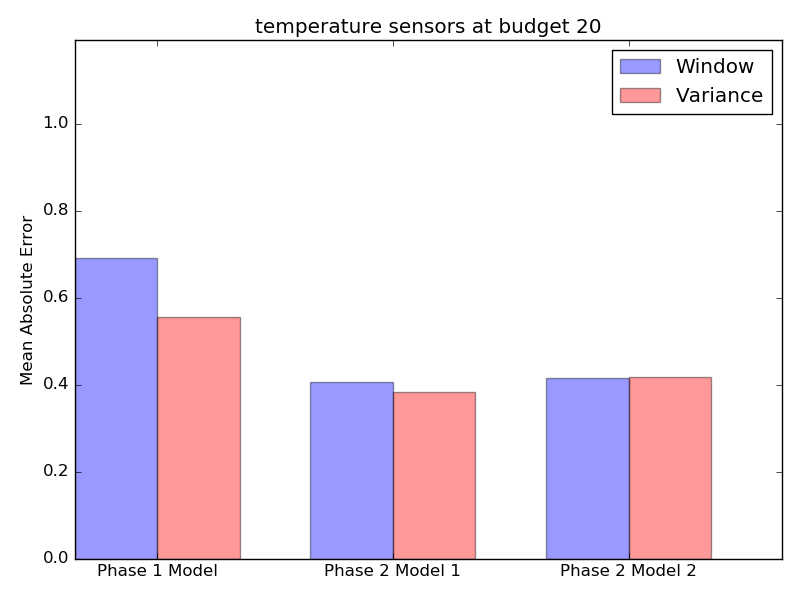
\includegraphics[scale=0.5]{temperature_20.png}
	\end{subfigure}
\end{figure}

\newpage

\begin{figure}[h!]
	\begin{subfigure}{\linewidth}
	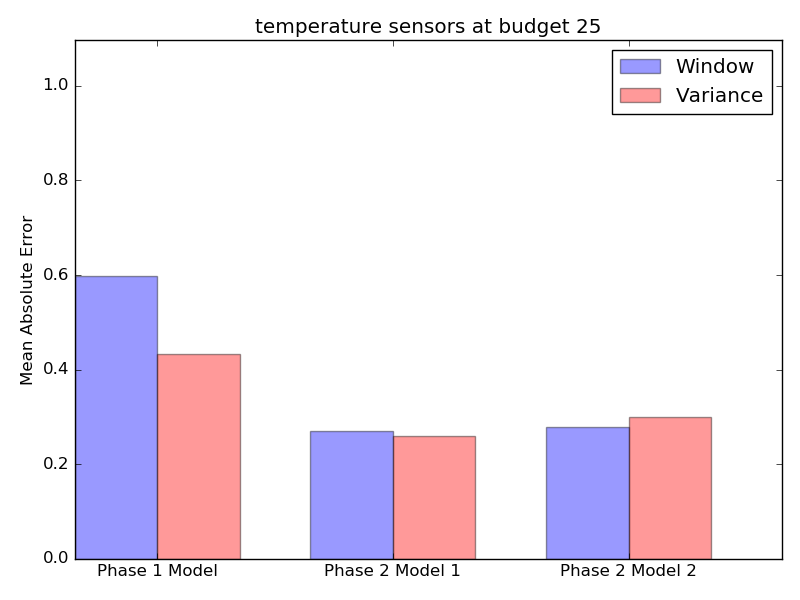
\includegraphics[scale=0.5]{temperature_25.png}
	\end{subfigure}
	\begin{subfigure}{\linewidth}
	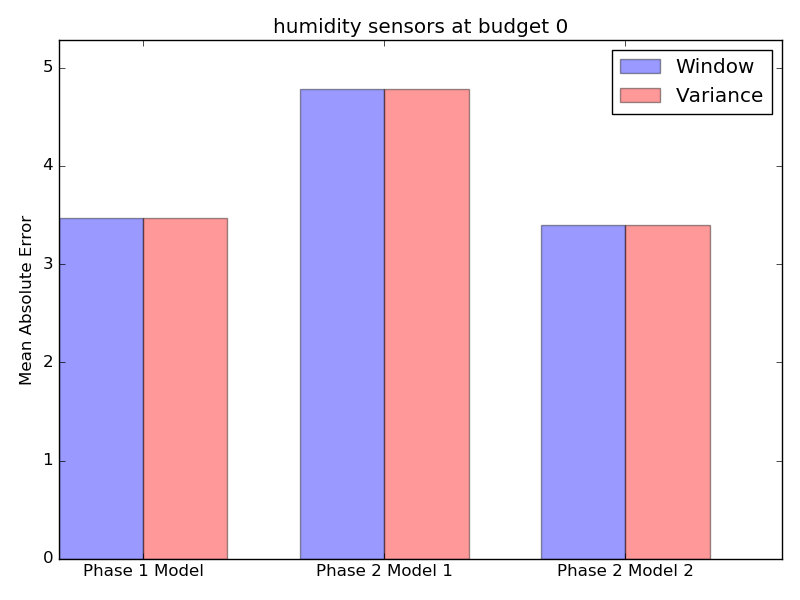
\includegraphics[scale=0.5]{humidity_0.png}
	\end{subfigure}
\end{figure}

\newpage

\begin{figure}[h!]
	\begin{subfigure}{\linewidth}
	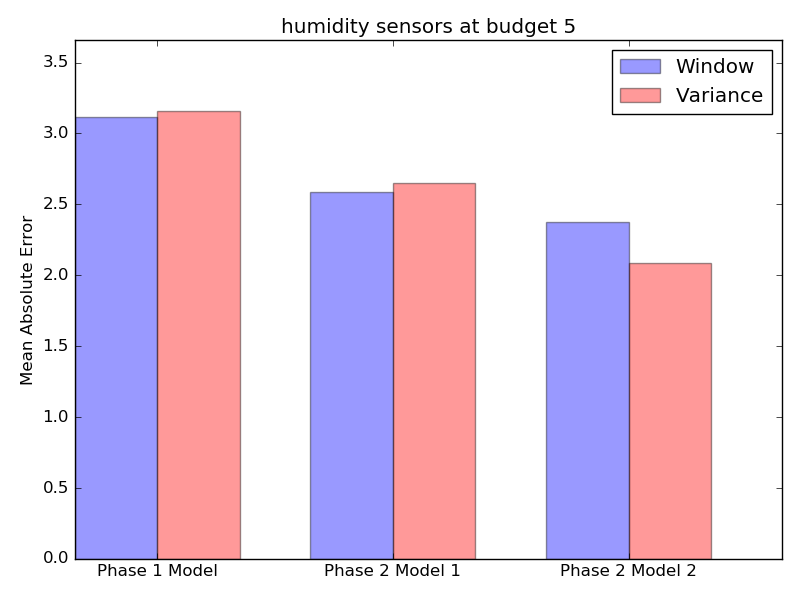
\includegraphics[scale=0.5]{humidity_5.png}
	\end{subfigure}
	\begin{subfigure}{\linewidth}
	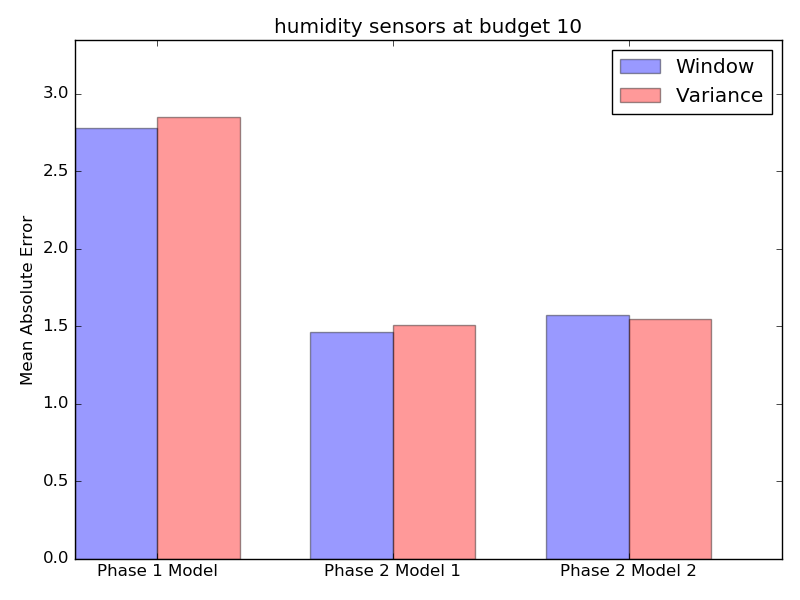
\includegraphics[scale=0.5]{humidity_10.png}
	\end{subfigure}
\end{figure}

\newpage

\begin{figure}[h!]
	\begin{subfigure}{\linewidth}
	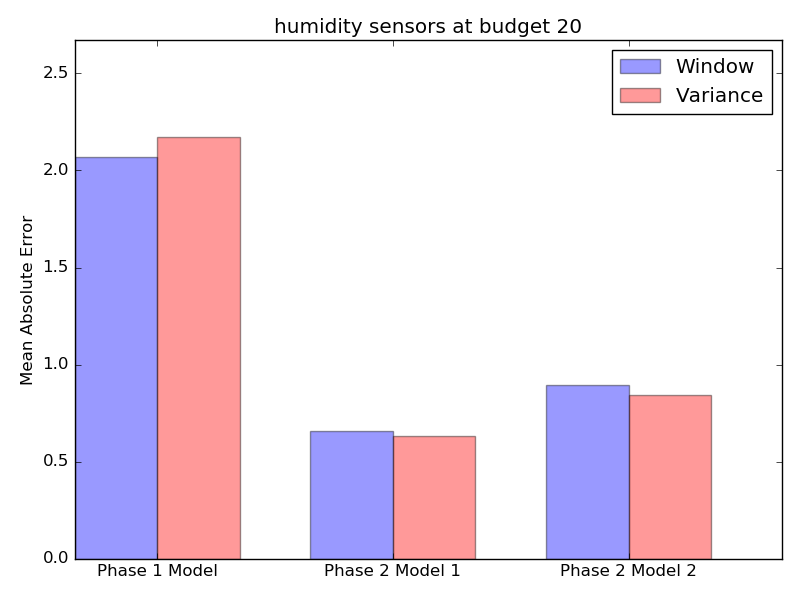
\includegraphics[scale=0.5]{humidity_20.png}
	\end{subfigure}
	\begin{subfigure}{\linewidth}
	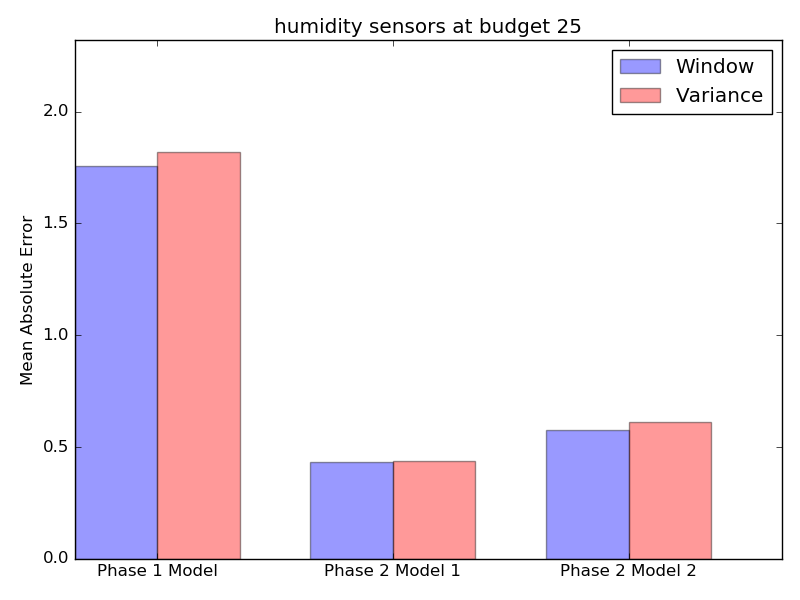
\includegraphics[scale=0.5]{humidity_25.png}
	\end{subfigure}
\end{figure}

\newpage

To do some verification first, all models do their
worst when the budget is 0 and their accuracy
increases as the budget increases. Also at
budget zero both inference methods have an equal
mean absolute error for each model which makes
sense, since nothing is observed.

At budget 0 for both humidity and temperature,
model 1 from phase 2 does worst. That makes sense
since each sensors parameters stay the same no
matter what the time is and it does not have the
granularity of of the phase 1 model or model 2
which basically have specific parameters tuned
for each timestamp in a day. This is also the
reason why model 2 and the phase 1 model have
more or less the same accuracy when the budget
is 0.

At budget 5 the temperature predictions
of model 1 are approaching the accuracy of
phase 1 model and model 2 as it gets some
help from the observed sensors. This happens
in the humidity sensor readings where model 1
not only catches up to the other two but it also
gets more accurate results than the phase 1
model.

The same trends as budget 5 are presented in
the graphs of budget 10, 20, and 25 (but all with even
more accurate results). Around budget 20 and then
at budget 25, we see that models 1 and 2 do
significantly better than the phase 1 model.
What is also surprising, is that model 1 actually
ends up doing better than model 2 in both
temperature and humidity readings at this point.
Model 2 is supposed to have a finer granularity
that would intuitively give more accurate results
than model 1. I still cannot make any conclusions
from these because our dataset is not that big
and varied.

As for the different active reference methods
used in our two new models, there really seems
to be no particular pattern and that is
understandable. Both methods do more or less
the same because depending on their budget
they will get data from all the sensors in a
specific period of time. In the Window method
that makes sense because it literally scans
through all the sensors. In the Variance method
that happens because once a sensor has been
observed the variance of its reading variance
is set to 0 and most probably it won't be
picked to be read any time soon since the
algorithm always chooses the sensors with
the highest variance.

\newpage

\section{More on Phase 3...}

\end{document}
